% This LaTeX document needs to be compiled with XeLaTeX.
\documentclass[10pt]{article}
\usepackage[utf8]{inputenc}
\usepackage{graphicx}
\usepackage[export]{adjustbox}
\graphicspath{ {./images/} }
\usepackage{amsmath}
\usepackage{amsfonts}
\usepackage{amssymb}
\usepackage[version=4]{mhchem}
\usepackage{stmaryrd}
\usepackage[fallback]{xeCJK}
\usepackage{polyglossia}
\usepackage{fontspec}
\setCJKmainfont{Noto Serif CJK TC}

\setmainlanguage{polish}
\setmainfont{CMU Serif}

\title{ARKUSZ PRÓBNEJ MATURY Z OPERONEM MATEMATYKA \\
 POZIOM PODSTAWOWY }

\author{LISTOPAD\\
2011}
\date{}


\begin{document}
\maketitle


\section*{Czas pracy: 170 minut}
\section*{Instrukcja dla zdającego}
\begin{enumerate}
  \item Sprawdź, czy arkusz egzaminacyjny zawiera 15 stron (zadania 1-34). Ewentualny brak zgłoś przewodniczącemu zespołu nadzorującego egzamin.
  \item Rozwiązania zadań i odpowiedzi zapisz w miejscu na to przeznaczonym.
  \item W rozwiązaniach zadań rachunkowych przedstaw tok rozumowania prowadzacy do ostatecznego wyniku.
  \item Pisz czytelnie. Używaj długopisu/pióra tylko z czarnym tuszem/atramentem.
  \item Nie używaj korektora, a błędne zapisy wyraźnie przekreśl.
  \item Zapisy w brudnopisie nie będą oceniane.
  \item Obok numeru każdego zadania podana jest maksymalna liczba punktów możliwych do uzyskania.
  \item Możesz korzystać z zestawu wzorów matematycznych, cyrkla i linijki oraz kalkulatora.
\end{enumerate}

Za rozwiązanie wszystkich zadań można otrzymać łącznie 50 punktów.

Życzymy powodzenia!

Wpisuje zdający przed rozpoczęciem pracy\\
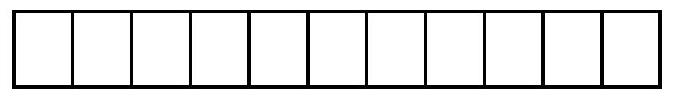
\includegraphics[max width=\textwidth, center]{2024_11_21_3a102e13f4b06a61f46fg-01}

PESEL ZDAJĄCEGO\\
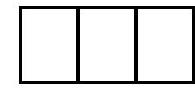
\includegraphics[max width=\textwidth, center]{2024_11_21_3a102e13f4b06a61f46fg-01(1)}

\section*{KOD}
ZDAJĄCEGO

\section*{ZADANIA ZAMKNIĘTE}
W zadaniach od 1. do 25. wybierz i zaznacz jedną poprawną odpowiedź.

\section*{Zadanie 1. (1 pkt)}
Największa liczba naturalna \(n\) spełniająca nierówność \(n<2 \pi-1\) to\\
A. 3\\
B. 5\\
C. 6\\
D. 0

\section*{Zadanie 2. (1 pkt)}
Liczba \(\frac{\sqrt[4]{16}+\sqrt[3]{3 \frac{3}{8}}}{\left(\frac{2}{7}\right)^{-1}}\) jest równa\\
A. -1\\
B. \(\frac{4}{49}\)\\
C. \(-2 \frac{1}{4}\)\\
D. 1

\section*{Zadanie 3. (1 pkt)}
Liczba \(\log 6\) jest równa\\
A. \(\log 2 \cdot \log 3\)\\
B. \(\frac{\log 12}{\log 2}\)\\
C. \(\log 2+\log 3\)\\
D. \(\log 2-\log 3\)

\section*{Zadanie 4. (1 pkt)}
20\% pewnej liczby jest o 16 mniejsze od tej liczby. Tą liczbą jest\\
A. 32\\
B. 20\\
C. -2\\
D. -20

\section*{Zadanie 5. (1 pkt)}
Rozwiązaniem równania \(-2=\frac{x-1}{x+2}\) jest liczba\\
A. -1\\
B. 1\\
C. 0\\
D. \(\frac{5}{3}\)

Zadanie 6. (1 pkt)\\
Większa z liczb spełniających równanie \(x^{2}+6 x+8=0\) to\\
A. 2\\
B. 4\\
C. -2\\
D. -4

\section*{Zadanie 7. (1 pkt)}
Przedział zaznaczony na osi liczbowej\\
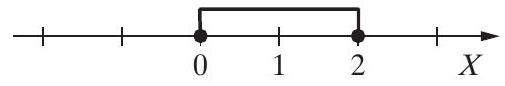
\includegraphics[max width=\textwidth, center]{2024_11_21_3a102e13f4b06a61f46fg-02}\\
jest zbiorem rozwiązań nierówności\\
A. \(|x+1| \leqslant 1\)\\
B. \(|x+1| \geqslant 2\)\\
C. \(|x-1| \geqslant 1\)\\
D. \(|x-1| \leqslant 1\)

\section*{BRUDNOPIS}
\begin{center}

\includegraphics[max width=\textwidth]{2024_11_21_3a102e13f4b06a61f46fg-03}
\end{center}

\section*{Zadanie 8. (1 pkt)}
Dziedziną funkcji \(f(x)=\left\{\begin{array}{ll}-2 x+1, & \text { gdy } x<1 \\ -x, & \text { gdy } 1 \leqslant x \leqslant 4\end{array}\right.\) jest zbiór\\
A. \((-\infty, 4\rangle\)\\
B. \(\langle 1,4\rangle\)\\
C. \(\langle 0,4\rangle\)\\
D. \((-\infty, 1)\)

\section*{Zadanie 9. (1 pkt)}
Funkcja liniowa \(f(x)=(m+2) x+2 m\) jest rosnąca, gdy\\
A. \(m<-2\)\\
B. \(m<2\)\\
C. \(m>-2\)\\
D. \(m>-4\)

\section*{Zadanie 10. (1 pkt)}
Rysunek przedstawia wykres funkcji \(y=f(x)\).\\
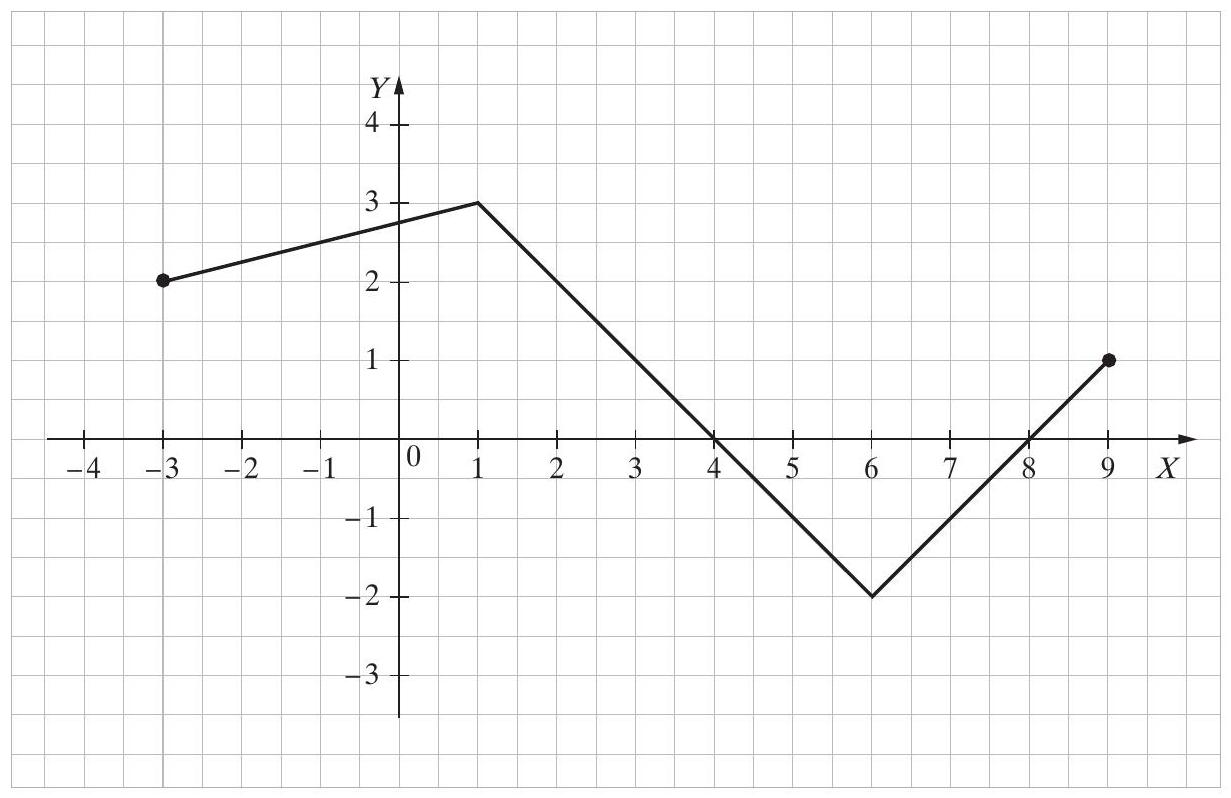
\includegraphics[max width=\textwidth, center]{2024_11_21_3a102e13f4b06a61f46fg-04}

Funkcja jest malejąca w przedziale\\
A. \(\langle 0,4\rangle\)\\
B. \(\langle 1,6\rangle\)\\
C. \(\langle 0,6\rangle\)\\
D. \(\langle-2,4\rangle\)

\section*{Zadanie 11. (1 pkt)}
Punkt \(P=(a+1,2)\) należy do wykresu funkcji \(f(x)=\frac{4}{x}\). Liczba \(a\) jest równa\\
A. 0\\
B. -1\\
C. 2\\
D. 1

\section*{Zadanie 12. (1 pkt)}
Do zbioru rozwiązań nierówności \(9 \leqslant x^{2}\) należy liczba\\
A. -2\\
B. 0\\
C. -3\\
D. 2

\section*{BRUDNOPIS}
\begin{center}

\includegraphics[max width=\textwidth]{2024_11_21_3a102e13f4b06a61f46fg-05}
\end{center}

\section*{Zadanie 13. (1 pkt)}
Wybierz i zaznacz równanie opisujące prostą prostopadłą do prostej o równaniu \(y=\frac{1}{2} x+1\).\\
A. \(y=-2 x+1\)\\
B. \(y=0,5 x-1\)\\
C. \(y=-\frac{1}{2} x+1\)\\
D. \(y=2 x-1\)

\section*{Zadanie 14. (1 pkt)}
Liczby \(x, 4, x+2\) są w podanej kolejności drugim, trzecim i czwartym wyrazem ciągu arytmetycznego. Wówczas liczba \(x\) jest równa\\
A. 2\\
B. 3\\
C. 6\\
D. 1

\section*{Zadanie 15. (1 pkt)}
W ciagu geometrycznym \(\left(a_{n}\right)\) są dane: \(a_{2}=-1, q=-2\). Suma czterech kolejnych początkowych wyrazów tego ciągu jest równa\\
A. 2,5\\
B. \(-7,5\)\\
C. \(-2,5\)\\
D. 7,5

\section*{Zadanie 16. (1 pkt)}
Kąt \(\alpha\) jest ostry i \(\sin \alpha=\frac{2}{5}\). Wówczas\\
A. \(\cos \alpha=\sin \alpha\)\\
B. \(\cos \alpha>\sin \alpha\)\\
C. \(\cos \alpha<\sin \alpha\)\\
D. \(\cos \alpha=1-\sin \alpha\)

\section*{Zadanie 17. (1 pkt)}
Dane są wielomiany \(W(x)=x^{4}-1\) oraz \(V(x)=x^{4}+1\). Stopień wielomianu \(W(x)+V(x)\) jest równy\\
A. 4\\
B. 8\\
C. 16\\
D. 0

\section*{Zadanie 18. (1 pkt)}
Mediana danych: \(-4,2,6,0,1\) jest równa\\
A. 6\\
B. 0\\
C. 2,5\\
D. 1

\section*{Zadanie 19. (1 pkt)}
Liczba punktów wspólnych okręgu o równaniu \((x-1)^{2}+y^{2}=4 \mathrm{z}\) prostą o równaniu \(y=-1\) jest równa\\
A. 0\\
B. 1\\
C. 2\\
D. 3

\section*{Zadanie 20. (1 pkt)}
Punkty \(A=(-2,-1)\) i \(B=(2,2)\) są wierzchołkami trójkąta równobocznego \(A B C\). Wysokość tego trójkąta jest równa\\
A. 2,5\\
B. \(2 \sqrt{3}\)\\
C. \(5 \sqrt{3}\)\\
D. \(2,5 \sqrt{3}\)

\section*{BRUDNOPIS}
\begin{center}

\includegraphics[max width=\textwidth]{2024_11_21_3a102e13f4b06a61f46fg-07}
\end{center}

\section*{Zadanie 21. (1 pkt)}
Dany jest okragg o środku w punkcie \(S\). Miara kąta \(\alpha\) jest równa \(70^{\circ}\).\\
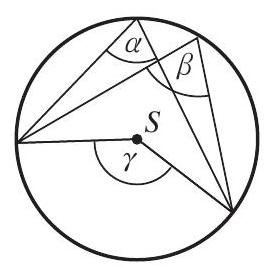
\includegraphics[max width=\textwidth, center]{2024_11_21_3a102e13f4b06a61f46fg-08(1)}

Suma miar kątów \(\beta\) i \(\gamma\) jest równa\\
A. \(180^{\circ}\)\\
B. \(210^{\circ}\)\\
C. \(70^{\circ}\)\\
D. \(140^{\circ}\)

\section*{Zadanie 22. (1 pkt)}
Trapez jest prostokątny. Trójkąty podobne \(A B D\) i \(C B D\) są równoramienne.\\
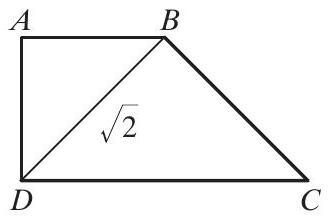
\includegraphics[max width=\textwidth, center]{2024_11_21_3a102e13f4b06a61f46fg-08}

Obwód trapezu jest równy\\
A. \(4+2 \sqrt{2}\)\\
B. \(2 \sqrt{2}\)\\
C. \(4+\sqrt{2}\)\\
D. 4

\section*{Zadanie 23. (1 pkt)}
Graniastosłup ma \(2 n+6\) wierzchołków. Liczba wszystkich krawędzi tego graniastosłupa jest równa\\
A. \(n+3\)\\
B. \(4 n+8\)\\
C. \(6 n+18\)\\
D. \(3 n+9\)

\section*{Zadanie 24. (1 pkt)}
Tworząca stożka jest o 2 dłuższa od promienia podstawy. Pole powierzchni bocznej tego stożka jest równe \(15 \pi\). Tworząca stożka ma zatem długość\\
A. 1\\
B. 5\\
C. 3\\
D. 15

\section*{Zadanie 25. (1 pkt)}
Cztery dziewczynki i sześciu chłopców siedzą na tym samym pniu zwalonego dębu. Dziewczynki siedzą obok siebie i chłopcy również siedzą obok siebie. Wszystkich możliwych sposobów posadzenia dzieci w ten sposób jest\\
A. \(4 \cdot 6\)\\
B. \(2 \cdot 4 \cdot 1 \cdot 2 \cdot 3 \cdot 4 \cdot 5 \cdot 6\)\\
C. \(1 \cdot 2 \cdot 3 \cdot 4 \cdot 6 \cdot 5 \cdot 4 \cdot 3 \cdot 2 \cdot 1\)\\
D. \(1 \cdot 2 \cdot 3 \cdot 4 \cdot 6 \cdot 5 \cdot 4 \cdot 3 \cdot 2 \cdot 1 \cdot 2\)

\section*{BRUDNOPIS}
\begin{center}

\includegraphics[max width=\textwidth]{2024_11_21_3a102e13f4b06a61f46fg-09}
\end{center}

\section*{ZADANIA OTWARTE}
\section*{Rozwiązania zadań o numerach od 26. do 34. należy zapisać w wyznaczonych miejscach pod treścią zadania.}
\section*{Zadanie 26. (2 pkt)}
Napisz równanie prostej równoległej do prostej o równaniu \(-3 x+y-4=0\) i przechodzącej przez punkt \(P=(-1,-4)\).\\

\includegraphics[max width=\textwidth, center]{2024_11_21_3a102e13f4b06a61f46fg-10(1)}

Odpowiedź: \(\qquad\)

\section*{Zadanie 27. (2 pkt)}
W trójkącie prostokątnym jedna z przyprostokątnych ma długość \(a\). Kąt ostry przy tym boku ma miarę \(\alpha\). Wykaż, że \(\sin \alpha+\cos \alpha>1\).\\

\includegraphics[max width=\textwidth, center]{2024_11_21_3a102e13f4b06a61f46fg-10}

\section*{Zadanie 28. (2 pkt)}
Wykaż, że przekątna prostopadłościanu o krawędziach długości \(a, b, c\) ma długość \(\sqrt{a^{2}+b^{2}+c^{2}}\).\\

\includegraphics[max width=\textwidth, center]{2024_11_21_3a102e13f4b06a61f46fg-11}

\section*{Zadanie 29. (2 pkt)}
Rozwiąż nierówność \(x^{2}+5 x \leqslant 6\).\\

\includegraphics[max width=\textwidth, center]{2024_11_21_3a102e13f4b06a61f46fg-11(1)}

Odpowiedź: \(\qquad\)

\section*{Zadanie 30. (2 pkt)}
Wiadomo, że \(A\) i \(B\) są takimi zdarzeniami losowymi zawartymi w \(\Omega\), że \(P(A)=0,7, P(B)=0,6\) i \(P(A \cup B)=0,8\). Oblicz \(P(A \cap B)\).\\

\includegraphics[max width=\textwidth, center]{2024_11_21_3a102e13f4b06a61f46fg-12}

Odpowiedź: \(\qquad\)

\section*{Zadanie 31. (2 pkt)}
Przekątna równoległoboku ma długość 10 cm i tworzy z krótszym bokiem kąt prosty, a z dłuższym bokiem kąt \(30^{\circ}\). Oblicz długość krótszego boku tego równoległoboku.

\begin{center}
\begin{tabular}{|c|c|c|c|c|c|c|c|c|c|c|c|c|c|c|c|c|c|c|c|c|c|c|c|c|c|c|c|c|c|}
\hline
 &  &  &  &  &  &  &  &  &  &  &  &  &  &  &  &  &  &  &  &  &  &  &  &  &  &  &  &  &  \\
\hline
 &  &  &  &  &  &  &  &  &  &  &  &  &  &  &  &  &  &  &  &  &  &  &  &  &  &  &  &  &  \\
\hline
 &  &  &  &  &  &  &  &  &  &  &  &  &  &  &  &  &  &  &  &  &  &  &  &  &  &  &  &  &  \\
\hline
 &  &  &  &  &  &  &  &  &  &  &  &  &  &  &  &  &  &  &  &  &  &  &  &  &  &  &  &  &  \\
\hline
 &  &  &  &  &  &  &  &  &  &  &  &  &  &  &  &  &  &  &  &  &  &  &  &  &  &  &  &  &  \\
\hline
 &  &  &  &  &  &  &  &  &  &  &  &  &  &  &  &  &  &  &  &  &  &  &  &  &  &  &  &  &  \\
\hline
 &  &  &  &  &  &  &  &  &  &  &  &  &  &  &  &  &  &  &  &  &  &  &  &  &  &  &  &  &  \\
\hline
 &  &  &  &  &  &  &  &  &  &  &  &  &  &  &  &  &  &  &  &  &  &  &  &  &  &  &  &  &  \\
\hline
 &  &  &  &  &  &  &  &  &  &  &  &  &  &  &  &  &  &  &  &  &  &  &  &  &  &  &  &  &  \\
\hline
 &  &  &  &  &  &  &  &  &  &  &  &  &  &  &  &  &  &  &  &  &  &  &  &  &  &  &  &  &  \\
\hline
 &  &  &  &  &  &  &  &  &  &  &  &  &  &  &  &  &  &  &  &  &  &  &  &  &  &  &  &  &  \\
\hline
 &  &  &  &  &  &  &  &  &  &  &  &  &  &  &  &  &  &  &  &  &  &  &  &  &  &  &  &  &  \\
\hline
 &  &  &  &  &  &  &  &  &  &  &  &  &  &  &  &  &  &  &  &  &  &  &  &  &  &  &  &  &  \\
\hline
 &  &  &  &  &  &  &  &  &  &  &  &  &  &  &  &  &  &  &  &  &  &  &  &  &  &  &  &  &  \\
\hline
 &  &  &  &  &  &  &  &  &  &  &  &  &  &  &  &  &  &  &  &  &  &  &  &  &  &  &  &  &  \\
\hline
 &  &  &  &  &  &  &  &  &  &  &  &  &  &  &  &  &  &  &  &  &  &  &  &  &  &  &  &  &  \\
\hline
 &  &  &  &  &  &  &  &  &  &  &  &  &  &  &  &  &  &  &  &  &  &  &  &  &  &  &  &  &  \\
\hline
 &  &  &  &  &  &  &  &  &  &  &  &  &  &  &  &  &  &  &  &  &  &  &  &  &  &  &  &  &  \\
\hline
 &  &  &  &  &  &  &  &  &  &  &  &  &  &  &  &  &  &  &  &  &  &  &  &  &  &  &  &  &  \\
\hline
 &  &  &  &  &  &  &  &  &  &  &  &  &  &  &  &  &  &  &  &  &  &  &  &  &  &  &  &  &  \\
\hline
\end{tabular}
\end{center}

Odpowiedź: \(\qquad\)

\section*{Zadanie 32. (4 pkt)}
Okrąg wpisany w trójkąt prostokątny \(A B C\) jest styczny do przeciwprostokątnej \(A B\) w punkcie \(K\). Wiadomo, że \(|A K|=4\) i \(|K B|=6\). Oblicz promień tego okręgu.\\
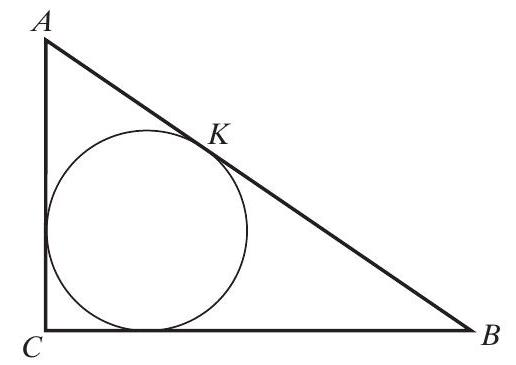
\includegraphics[max width=\textwidth, center]{2024_11_21_3a102e13f4b06a61f46fg-13}\\

\includegraphics[max width=\textwidth, center]{2024_11_21_3a102e13f4b06a61f46fg-13(1)}

Odpowiedź: \(\qquad\)

\section*{Zadanie 33. (4 pkt)}
Rzucamy dwukrotnie kostką do gry. Jakie jest prawdopodobieństwo tego, że liczba oczek otrzymana w pierwszym rzucie jest większa od liczby oczek otrzymanej w drugim rzucie?

\begin{center}
\begin{tabular}{|c|c|c|c|c|c|c|c|c|c|c|c|c|c|c|c|c|c|c|c|c|c|c|c|c|c|c|c|c|c|c|c|}
\hline
 &  &  &  &  &  &  &  &  &  &  &  &  &  &  &  &  &  &  &  &  &  &  &  &  &  &  &  &  &  &  &  \\
\hline
 &  &  &  &  &  &  &  &  &  &  &  &  &  &  &  &  &  &  &  &  &  &  &  &  &  &  &  &  &  &  &  \\
\hline
 &  &  &  &  &  &  &  &  &  &  &  &  &  &  &  &  &  &  &  &  &  &  &  &  &  &  &  &  &  &  &  \\
\hline
 &  &  &  &  &  &  &  &  &  &  &  &  &  &  &  &  &  &  &  &  &  &  &  &  &  &  &  &  &  &  &  \\
\hline
- &  &  &  &  &  &  &  &  &  &  &  &  &  &  &  &  &  &  &  &  &  &  &  &  &  &  &  &  &  &  &  \\
\hline
 &  &  &  &  &  &  &  &  &  &  &  &  &  &  &  &  &  &  &  &  &  &  &  &  &  &  &  &  &  &  &  \\
\hline
到 &  &  &  &  &  &  &  &  &  &  &  &  &  &  &  &  &  &  &  &  &  &  &  &  &  &  &  &  &  &  &  \\
\hline
 &  &  &  &  &  &  &  &  &  &  &  &  &  &  &  &  &  &  &  &  &  &  &  &  &  &  &  &  &  &  &  \\
\hline
 &  &  &  &  &  &  &  &  &  &  &  &  &  &  &  &  &  &  &  &  &  &  &  &  &  &  &  &  &  &  &  \\
\hline
 &  &  &  &  &  &  &  &  &  &  &  &  &  &  &  &  &  &  &  &  &  &  &  &  &  &  &  &  &  &  &  \\
\hline
 &  &  &  &  &  &  &  &  &  &  &  &  &  &  &  &  &  &  &  &  &  &  &  &  &  &  &  &  &  &  &  \\
\hline
 &  &  &  &  &  &  &  &  &  &  &  &  &  &  &  &  &  &  &  &  &  &  &  &  &  &  &  &  &  &  &  \\
\hline
 &  &  &  &  &  &  &  &  &  &  &  &  &  &  &  &  &  &  &  &  &  &  &  &  &  &  &  &  &  &  &  \\
\hline
 &  &  &  &  &  &  &  &  &  &  &  &  &  &  &  &  &  &  &  &  &  &  &  &  &  &  &  &  &  &  &  \\
\hline
 &  &  &  &  &  &  &  &  &  &  &  &  &  &  &  &  &  &  &  &  &  &  &  &  &  &  &  &  &  &  &  \\
\hline
 &  &  &  &  &  &  &  &  &  &  &  &  &  &  &  &  &  &  &  &  &  &  &  &  &  &  &  &  &  &  &  \\
\hline
 &  &  &  &  &  &  &  &  &  &  &  &  &  &  &  &  &  &  &  &  &  &  &  &  &  &  &  &  &  &  &  \\
\hline
\end{tabular}
\end{center}

Odpowiedź: \(\qquad\)

\section*{Zadanie 34. (5 pkt)}
Piramida ma kształt ostrosłupa prawidłowego czworokątnego, którego wysokość jest równa 6, a długość krawędzi bocznej jest równa \(2 \sqrt{15}\). Oblicz miarę kąta nachylenia ściany bocznej piramidy do podstawy.\\

\includegraphics[max width=\textwidth, center]{2024_11_21_3a102e13f4b06a61f46fg-14}

Odpowiedź: \(\qquad\)

\section*{BRUDNOPIS (nie podlega ocenie)}

\end{document}